\section{Discussion}\label{discussion}

% original
Many non-trivial problems in materials science, and in science more broadly, are explained not through a single constitutive relationship, but through a combination of contributing physics.

% Figure~\ref{fig:stress} shows an artificial dataset constructed to replicate the impact of yield stress in a two-phase, solid-solution strengthened alloy system. Using a combination of composite theory for the contribution of flow stress, {\color{red} NAME} solid solution \cite{solid solution}, and Hall-Petch \cite{Hall-Petch} strengthening, the expected yield stress is
%
% \begin{equation}
% 	\sigma_y = F_v^A \sigma_f^A + F_v^B \sigma_f^B + \sum_i C_i [x_i]^{2/3} + \sum_j k_j d_j^{-1/2} + \ldots
% \end{equation}
%
% \noindent with free parameters \\[2ex]
% \begin{conditions}
% 	F_v^i  & Volume fraction of phase $i$ \\
% 	$[x_i]$  & Concentration of solute $i$ \\
% 	d_j    & Average grain diameter of phase $j$
% \end{conditions}
% \\[2ex]
% \noindent and fixed parameters \\[2ex]
% \begin{conditions}
% 	\sigma_f^i & Flow stress of phase $i$ \\
% 	C_i        & Solid solution strengthening coefficient for solute species $i$ \\
% 	k_j        & Hall-Petch strengthening coefficient for phase $j$
% \end{tabular}
% \\[2ex]

% The goal is to iteratively improve on this constitutive model, one term at a time, and monitor the effect on the residuals between the predicted yield, $\hat{\sigma_y}$ and the actual yield $\sigma_y$.
The goal of this approach is to identify the coefficients of a hypothesized constitutive relationship, coefficients that capture the specific physics of a process, through a least-squares fit between the covector space of a neural network series expansion, $\boldsymbol{\alpha}(\boldsymbol{\theta})$, which is a function of the model parameters, and the covector space of the constitutive relationship, $\boldsymbol{\beta}(C_k)$, which is a function of the physical constants of the model.

It may be useful to introduce a schematic that not only frames the hypothesis, but also graphically registers key details of the methods section of this paper.  Such a figure is presented in Figure~\ref{fig:nn-2}


\begin{figure}[htbp]
\begin{center}
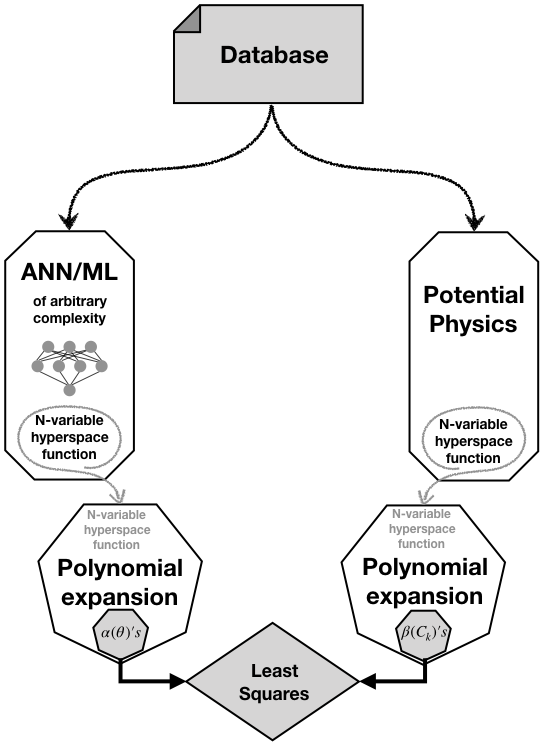
\includegraphics[width=0.4\textwidth]{fig/Schematic-02}
\caption{Schematic of the logic of the approach. The schematic could easily be expanded to show additional details and complexity on both the ANN/ML pathway and the potential physics pathway, including, for example, data selectors, physical dependencies. Similarly, the permutation of multiple architectures and postulated physics could be graphically represented, which would better represent the practical use of this approach.}
\label{fig:nn-2}
\end{center}
\end{figure}


% Find \alpha_k for neural network (NN) expansion
% Find \beta_k for constitutive relationship (CR) expansion
% Solve for C_k through fit (least-squares for now) of \alpha_k to \beta_k
Having fit the model parameters, $\boldsymbol{\theta}$, on a vector space spanned by the column vectors of ${\bf x}$, the coefficients (the covector basis) of the neural network expansion, $\boldsymbol{\alpha}(\boldsymbol{\theta})$, capture the functional relationship between the input space and the response space, both affine and non-linear contributions, introduced through those parameters, $\boldsymbol{\theta}$, and the coefficient generating functions for the activation, e.g. Equations~\ref{eqn:ReLU generating function} (Rectified Linear Unit, ReLU) and \ref{eqn:softmax generating function} (softmax), respectively.

Naturally, the activation generating functions must match the activation function chosen in the neural network model architecture. Equation~\ref{eqn:ReLU generating function} is derived for ReLU activation, the most common hidden layer activation. (Generating functions for other activations are provided in the appendix.) In addition to the hidden layers, activation functions must also be chosen for the output layer. The two most common output activations are linear (Eq.~\ref{eqn:linear generating function}) and softmax (Eq.~\ref{eqn:softmax generating function}) for regression and classification, respectively.

% possible because \alpha and \beta both span the same subspace.
\begin{condition}
    Both the neural network and the constitutive relationship must depend on the same independent variables.
\end{condition}
That is, they must be described on the same basis vectors. The fit between the coefficients of the neural network expansion--$\boldsymbol{\alpha}$, the covector space of the neural network's basis vectors--and the coefficients of the series expansion of the constitutive relationship (its covector space, $\boldsymbol{\beta}$) is only possible because both span the same subspace and share a common description of the solution within that subspace, that is, the covector spaces are colinear. That is, suppose that $A$ maps between a vector space and its covector space. If $A: A(X) = X^*$ and $A: A(Y) = Y^*$, then $X^* = Y^*$ if and only if $X = Y$.

One example of the proposed method is provided, where the mapping of the polynomial expansions for both the neural network and potential physics is performed for yield strength, which is known to depend on intrinsic flow stress, as well as solute and grain size contributions:

\begin{equation}
    \sigma_y = \sigma_f + \sum_{k=0}^\infty \sum_{l_1=0}^k \binom{k}{l_1, l_2} \left( a_k \prod_{m=1}^2 ({\bf S}_\text{solute})_m^{l_m} + b_k \prod_{m=1}^2 ({\bf S}_\text{Hall-Petch})_m^{l_m} \right) \prod_{m=1}^2{\bf x}_m^{l_m}
\end{equation}

where
\begin{conditions}
    \sigma_f & Matrix flow stress. \\
    a_k & Coefficient generating function for $x^{2/3}$. \\
    b_k & Coefficient generating function for $x^{-1/2}$. \\
    {\bf S}_\text{solute} & Selection vector/matrix for choosing the solute concentration from the input vector. \\
    {\bf S}_\text{Hall-Petch} & Selection vector/matrix for choosing the grain size from the input vector. \\
    {\bf x} = ([c], d) & concentration of a solute and grain size, respectively.
\end{conditions}

It should be noted here that this common basis is a function of the length (dimension) of the input vector and of the order of the expansion. Therefore, two series will share the same basis vector and the same covector space if and only if they are taken to the same order. In addition, because there is no guarantee that the input vector space directions are orthogonal, there is no guarantee that the cross-term interactions will vanish and, therefore, must be included explicitly. This expansion includes all cross-terms and, through the element-wise exponentiation, also explicitly captures all combinations of powers of all cross-terms.

% dimensional sufficiency
{\color{red} TBW. This must answer the question: how do we know if we've measured the right things--not the number of measurements, but that we have enough information? How do we know that the solution has converged? Example: A model is to be fit to the number of cakes produced by a bakery. If we are given weights of flour and sugar and number of eggs, our model can accurately tell us the \emph{volume} of cakes produced, but not the number. If this bakery makes cupcakes, but the model is trained across a spectrum of bakers, such as purveyors of wedding cakes and catering companies who work with large sheet cakes, then our dimensions (flour, sugar, eggs) are insufficient to fit the number of cakes produced. If, however, we also include number of orders and revenue, some information about the \emph{quanta} of cakes is baked into those two additional dimensions (sorry, I couldn't help myself). Therefore, a model based only on (flour, sugar, eggs) is dimensionally insufficient, but a model based on (flour, sugar, eggs, order size, revenue) is dimensionally sufficient.

This is a broader question that may be beyond the scope of this paper. Let's return to this if, after completing the first pass, we feel that this can be addressed by what we've done.}

% comment on the distance metric
% The Euclidean ($L_2\textrm{-norm}$) distance is used in optimizations, such as the training of neural networks and other machine learning algorithms, through the mean-square error,
% \begin{equation*}
%     \argmin_{\boldsymbol{\theta}} \|{\bf y} - \boldsymbol{\theta}{\bf x}\|.
% \end{equation*}
% However because of the curse of dimensionality,~\cite{curse of dimensionality reference?} the $L_2\textrm{-norm}$ is not a desirable metric in high-dimensional spaces.

This leads to a seven-step process for systematically and incrementally extracting physics information from an ANN:
\begin{enumerate}
	\item Collect data--features and targets--for which relationships are expected to exist.
	\item Design and train a fully dense multi-layer perceptron network (ANN).
	\item Build a power series expansion from the architecture of this ANN, using Equations~(\ref{eqn:sigmoid zeta expansion}) and (\ref{eqn:ANN power series coefficient generating function}) to populate the coefficients using the trained weights from the neural network.
	\item Hypothesize a constitutive relationship between the feature space and the target space. \label{item:hypothesis}
	\item Recast the terms in the hypothesis function from \#\ref{item:hypothesis} as power series expansions, creating power series coefficient generating functions that are functions of the constitutive model fitting parameters. An example of this process is provided below, and a table of select power series expansions relevant to materials research are provided in Table~(\ref{table:power series expansions}). \label{item:coefficients}
	\item Perform an optimization, \emph{e.g.} least squares, fit to find the fitting parameters from \#\ref{item:coefficients}
	\item Calculate the residuals of the ANN power series expansion coefficient vector, and from this residual vector, the error in the model. If the accuracy is sufficient for the application, stop; otherwise, expand the constitutive relationship from step \#\ref{item:hypothesis} and repeat.
\end{enumerate}

\subsection{Polynomial Expansion of a Vector Layer}
The polynomial expansion for the determination of coefficient is not limited to only scalar layers. It is possible to apply the same method presented here in this work to vectors and tensors. A more detailed and rigorous derivation for vector layers is provided in the Appendix of this work. Although a relatively simple approach has been provided in Section 3.2, the challenge is in finding the solutions to the index and power constraints.

%\noindent {\color{red} How does dropout affect this? It doesn't. Dropout simply sets specific $\boldsymbol\theta$ to zero, which is handled seamlessly in the previous treatment.}

\subsubsection{Interpretation}

\begin{equation*}
    s_k \theta^k \binom{k}{k_0, k_1, \cdots, k_i} \prod_{n=0}^{\infty} a_n^{k_n}
\end{equation*}

may be pulled out and added to the sum of $b_i$. In concise terms we have derived that

\begin{equation}
    b_i = \sum_{k=0}^{\infty} s_k \theta^k \sum_{\substack{k_0 + k_1 + \cdots + k_i = k \\ 0 k_0 + 1 k_1 + \cdots + i k_i = i}} \binom{k}{k_0, k_1, \cdots, k_i} \prod_{n=0}^{\infty} a_n^{k_n}.
	\label{eqn:scalar power series result}
\end{equation}

Thus, we have derived a tractable method of computing the coefficients of a power series after a linear and nonlinear transformation. We have included some worked examples of these coefficients in Appendix \ref{sec:worked scalar coeffs}.
%End of scalar coefficients derivation.%
